\chapter{Результаты работы} \label{ch5}
Предлагается построить симуляцию на основании реально существующего участка дороги в г. Москве.

\section{Анализ входных данных} \label{ch5:sec1}
\subsection{Карта исследуемого участка дороги}
\begin{figure}[!htbp]
		\centering
		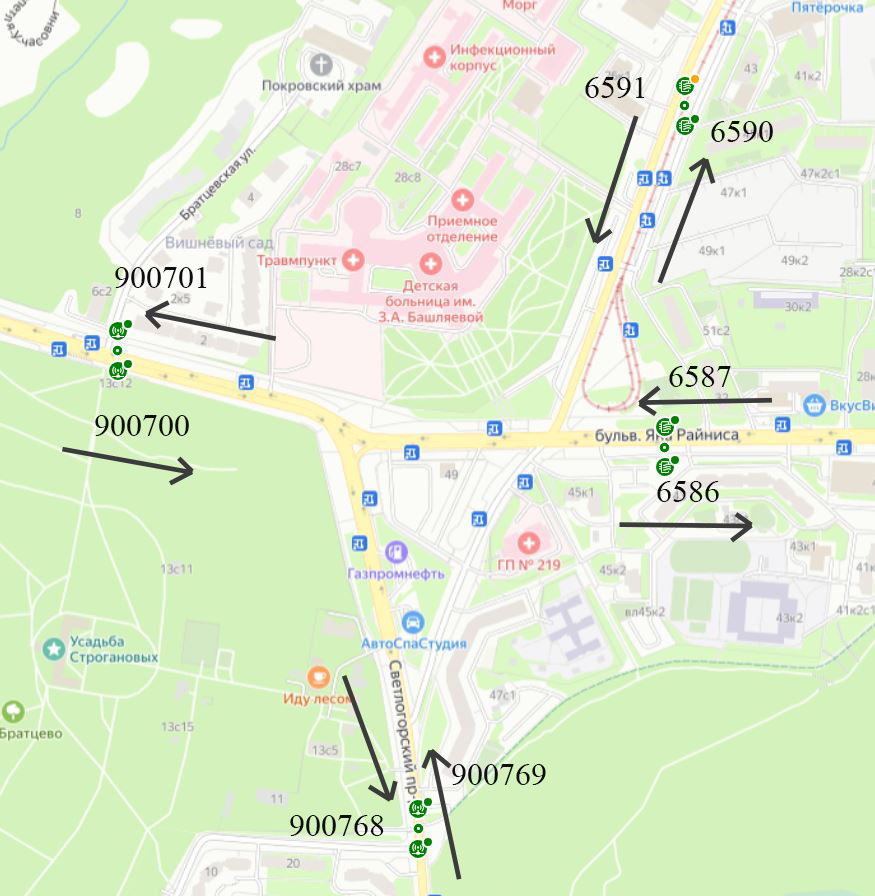
\includegraphics[height=0.5\textheight,valign=t]{my_folder/images//radiodetectors.JPG}
		
\captionsetup{justification=centering} %центрировать
	\caption{Участок дорожной карты с обозначением номеров радиодетекторов} 
\end{figure}

На \firef{fig:radiodetectors-map} номерами 1 и 2 обозначены светофорные объекты, регулирующие движение на представленных перекрестках.\\
Номерами со стрелками 900700, 6586 и т.д. обозначены номера детекторов.
На \firef{fig:detectors-mapping} указано расположение указано расположение радиодетекторов.
\newpage

\begin{figure}[!htbp]
	\centering
	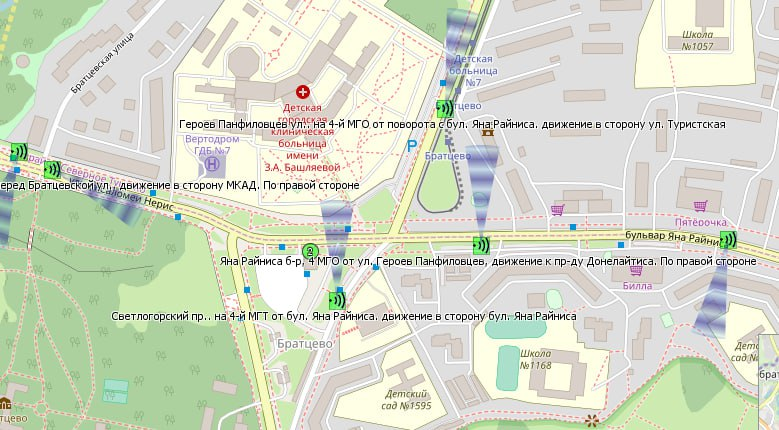
\includegraphics[height=0.3\textheight,valign=t]{my_folder/images//detectors-mapping.jpg}
	
\captionsetup{justification=centering} %центрировать
\caption{Местоположение детекторов на дороге}\label{fig:detectors-mapping}
\end{figure}

\begin{figure}[!htbp]
		\centering
		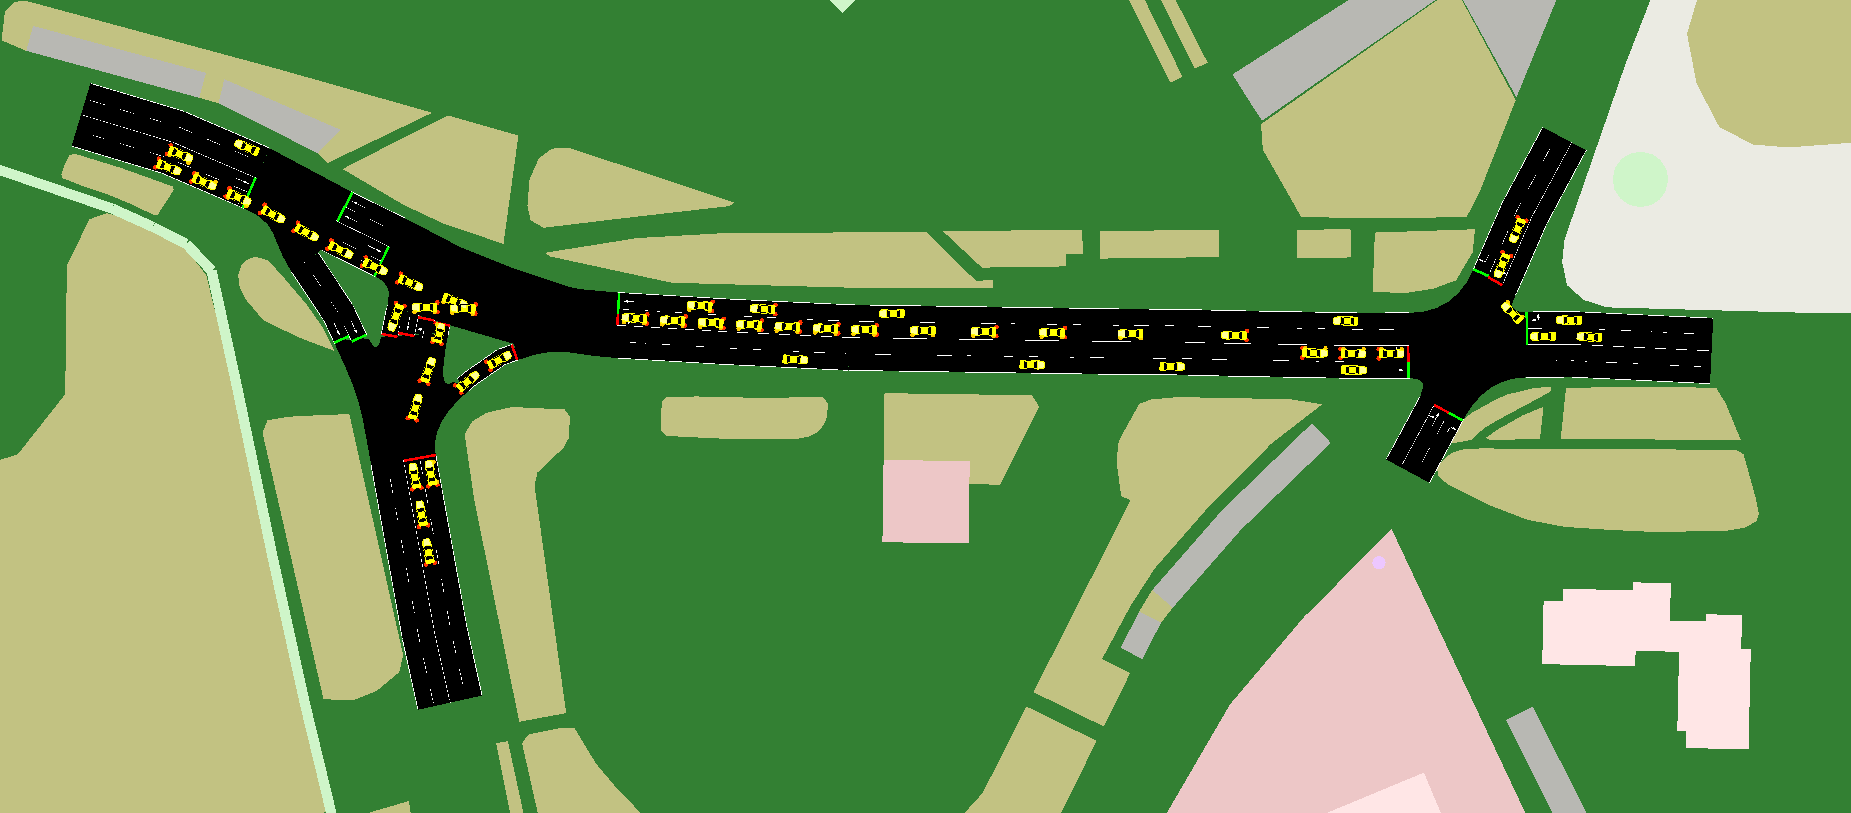
\includegraphics[height=0.3\textheight,valign=t]{my_folder/images//sumo-gui-roadmap.png}
		
\captionsetup{justification=centering} %центрировать
	\caption{Модель участка дороги на основе \firef{fig:radiodetectors-map}} 
\end{figure}

\newpage
На \firef{fig:detectors-setting} желтым обозначены позиции детекторов, содерщащих информацию о количестве машин в вершинах-источниках и вершинах-стоках.
\begin{figure}[!htbp]
    \centering
    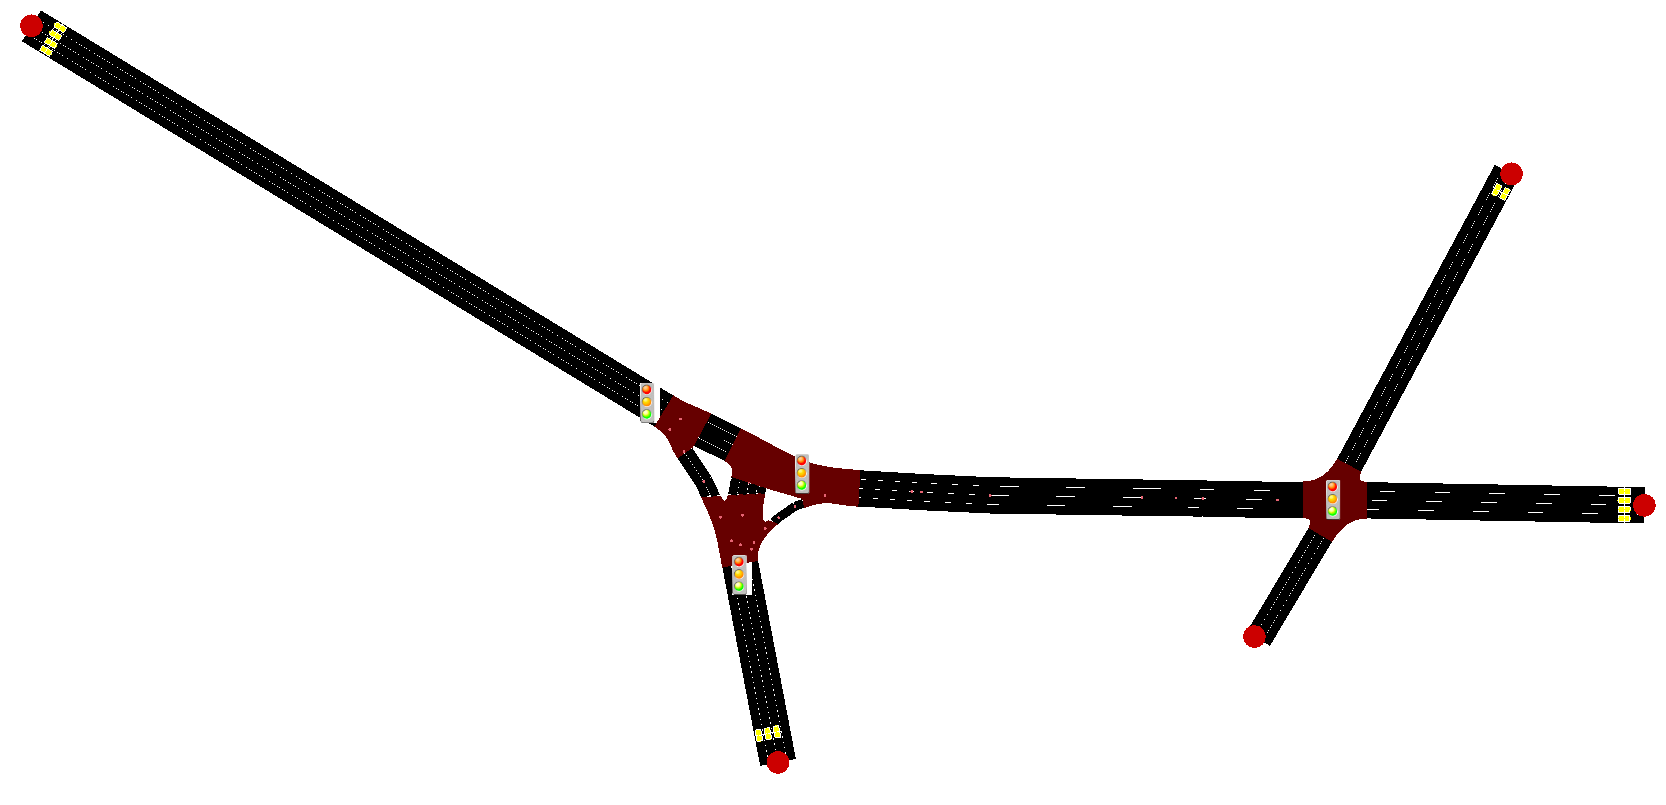
\includegraphics[height=0.2\textheight,valign=t]{my_folder/images//detectors-setting.png}
    
\captionsetup{justification=centering} %центрировать
\caption{Места расположения детекторов на карте}\label{fig:detectors-setting}
\end{figure}


\subsection{Определение состояний}
Информация о направлениях движения, регулируемых светофорными объектами 1 и 2, представлена в паспортах СО соответственно.\\
Отметим, что оптимизация фаз, связанных с движением пешеходов, не производится. Время, отведённое под движение пешеходов,взято как исходное константное значение из паспорта.

На \firef{fig:linked-phase-d} представлены направления пешеходного движения.\\
\begin{figure}[ht]
	\adjustbox{minipage=1.3em,valign=t}{\subcaption{}\label{fig:linked-phase-a}}%
	\begin{subfigure}[t]{\dimexpr.5\linewidth-1.3em\relax}
		\centering
		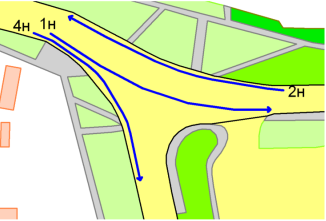
\includegraphics[width=.70\linewidth,valign=t]{my_folder/images/linked-0.png}
	\end{subfigure}
\hfill %выровнять по ширине
	\adjustbox{minipage=1.3em,valign=t}{\subcaption{}\label{fig:spbpu_sc-b}}%
	\begin{subfigure}[t]{\dimexpr.5\linewidth-1.3em\relax}
		\centering
		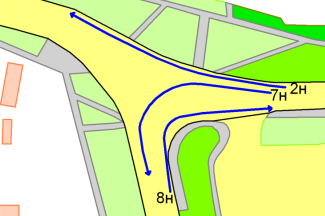
\includegraphics[width=.70\linewidth,valign=t]{my_folder/images/linked-1.png}
	\end{subfigure}
\\[20pt]
	\adjustbox{minipage=1.3em,valign=t}{\subcaption{}\label{fig:spbpu_sc-c}}%
\begin{subfigure}[t]{\dimexpr.5\linewidth-1.3em\relax}
	\centering
	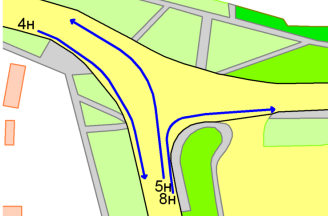
\includegraphics[width=.70\linewidth,valign=t]{my_folder/images/linked-2.png}
\end{subfigure}%
\hfill %выровнять по ширине
\adjustbox{minipage=1.3em,valign=t}{\subcaption{}\label{fig:spbpu_sc-d}}%
\begin{subfigure}[t]{\dimexpr.5\linewidth-1.3em\relax}
	\centering
	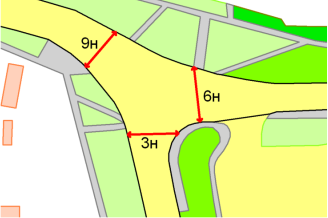
\includegraphics[width=.70\linewidth,valign=t]{my_folder/images/linked-red.png}
\end{subfigure}
\captionsetup{justification=centering} %центрировать
\caption{Направлениия движения СО 1} 
\label{fig:linked-phases}
\end{figure}

\newpage
На \firef{fig:separate-phase-c} представлены направления пешеходного движения.
\begin{figure}[ht]
	\adjustbox{minipage=1.3em,valign=t}{\subcaption{}\label{fig:separate-phase-a}}%
	\begin{subfigure}[t]{\dimexpr.5\linewidth-1.3em\relax}
		\centering
		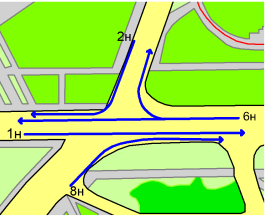
\includegraphics[width=.80\linewidth,valign=t]{my_folder/images/separate-0.png}
	\end{subfigure}
\hfill %выровнять по ширине
	\adjustbox{minipage=1.3em,valign=t}{\subcaption{}\label{fig:separate-phase-b}}%
	\begin{subfigure}[t]{\dimexpr.5\linewidth-1.3em\relax}
		\centering
		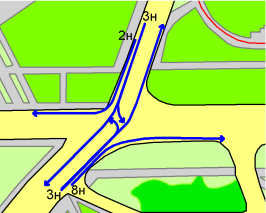
\includegraphics[width=.80\linewidth,valign=t]{my_folder/images/separate-1.png}
	\end{subfigure}
\\[20pt]
	\adjustbox{minipage=1.3em,valign=t}{\subcaption{}\label{fig:separate-phase-c}}%
\begin{subfigure}[t]{\dimexpr.5\linewidth-1.3em\relax}
	\centering
	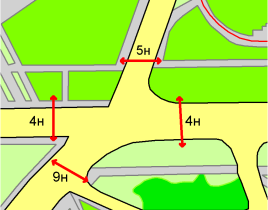
\includegraphics[width=.80\linewidth,valign=t]{my_folder/images/separate-red.png}
\end{subfigure}%
\hfill %выровнять по ширине
\adjustbox{minipage=1.3em,valign=t}{\subcaption{}\label{fig:separate-phase-d}}%
\begin{subfigure}[t]{\dimexpr.5\linewidth-1.3em\relax}
	\centering
	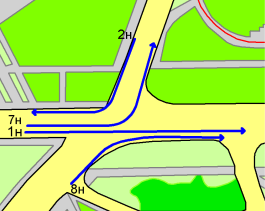
\includegraphics[width=.80\linewidth,valign=t]{my_folder/images/separate-2.png}
\end{subfigure}
\captionsetup{justification=centering} %центрировать
\caption{Направлениия движения СО 2} 
\label{fig:linked-phases}
\end{figure}

%\FloatBarrier % заставить рисунки и другие подвижные (float) элементы остановиться

\newpage
\section{Результаты оптимизации}
В таблице \taref{tab:opt-res} отображены результаты запусков алгоритмов оптимизации.\\
В заголовке таблицы использованы следующие обозначения:
\begin{itemize}
	\item Наз.алг - название алгоритма.
	\item $X_{opt}$ - решение задачи оптимизации \labelcref{eq:goal-function}.
	\item  $f(X_{opt})$ - значение ЦФ в $X_{opt}$, [c].
	\item $I$ - количество итераций (поколений, популяций).
	\item $N_{f}$ - количество подсчётов ЦФ.
	\item $T_{\text{общ}}$ - общее время работы алгоритма [c].
	\item $T_{i}$ - среднее время подсчётов ЦФ на текущей итерации [c].
	\item $N_{e}$ - количество машин, к концу симуляции завершивших намеченные маршруты.
\end{itemize}
Заметим, что на основе паспортов СО длительности фаз выглядят следующим образом:\begin{equation}
	X_{src} = [65, 35, 20, 40, 22, 34], \ f(X_{src}) = 73.42, \ N_{e} = 4767\label{eq:src}
\end{equation}
Количество машин, предзагруженных в симуляцию на основе данных с детекторов, $N_c = 5959$.\\
Временной интервал симуляции: 06:00-09:00, время по счётчику SUMO --begin 0 --end 10800 (3ч).\\
\noindent % for correct centering
\begin{minipage}{\textwidth}
	\vspace{\mfloatsep} % интервал 
	\centering\small
	\captionof{table}{Результаты работы алгоритмов оптимизации}%
	\label{tab:opt-res}
	\begin{tabular}{|l|l|l|l|l|l|l|l|}
	\hline
	Наз. алг.&$X_{opt}$&$f(X_{opt})$&$I$&$N_{f}$&$T_{\text{общ}}$&$T_{i}$&$N_{e}$\\
	\hline
	CMA-ES&[57, 43, 20, 42, 39, 36]&64.48&100&900&415.64&4.16&5506\\ \hline
	CMA-ES&[55, 37, 26, 33, 42, 34]&64.27&125&1125&509.29&4.07&5505\\ \hline
	CMA-ES&[58, 40, 20, 41, 41, 37]&62.62&125&1125&501.25&4.01&5376\\ \hline
	CMA-ES&[53, 39, 26, 42, 37, 38]&61.27&125&1125&519.67&4.16&5653\\ \hline
	CMA-ES&[59, 37, 22, 34, 37, 32]&63.85&250&2250&1004.94&4.02&5472\\ \hline
	CMA-ES&[58, 40, 20, 39, 32, 34]&65.36&250&2250&998.58&3.99&5314\\ \hline
	CMA-ES&[56, 35, 27, 25, 41, 38]&65.12&250&2250&985.96&3.94&5186\\ \hline
	ГА&[51, 38, 29, 32, 47, 40]&62.39&100&3281&1372.01&13.72&5407 \\ \hline
	ГА&[55, 43, 20, 52, 27, 38]&64.05&100&2945&1221.41&12.21&5114\\ \hline
	ГА&[60, 37, 21, 37, 37, 43]&63.83&100&3108&1281.66&12.82&5305\\ \hline
	ГА&[51, 34, 33, 39, 41, 37]&63.69&250&7545&3298.57&13.19&5624\\ \hline
	ГА&[57, 35, 23, 40, 38, 39]&64.75&250&7851&3305.79&13.22&5470\\ \hline
	ГА&[55, 34, 29, 29, 45, 43]&62.75&250&7568&3162.45&12.65&5295\\ \hline
	ГА&[58, 40, 20, 28, 47, 42]&62.77&300&8076&3396.7&11.32&5066\\ \hline
	МРЧ&[53, 39, 26, 28, 48, 43]&61.23&50&10150&3932.94&78.66&5221\\ \hline
	МРЧ&[50, 39, 29, 49, 34, 35]&60.04&50&10150&3917.7&78.35&5602\\ \hline
	МРЧ&[48, 42, 28, 50, 29, 39]&61.56&50&10150&3922.45&78.45&5358\\ \hline
	МРЧ&[52, 38, 28, 41, 39, 38]&60.2&75&15225&5881.12&78.41&5636\\ \hline
	МРЧ&[48, 38, 32, 46, 34, 38]&60.67&75&15225&6037.65&80.5&5581\\ \hline
	МРЧ&[55, 37, 26, 41, 41, 36]&60.16&75&15225&6262.81&83.5&5684\\ \hline
	МРЧ&[50, 38, 30, 51, 27, 40]&60.69&100&20300&8263.69&82.64&5252\\ \hline		
	\end{tabular}
\vspace{\mfloatsep} % интервал 
\normalsize %восстанавливаем шрифт 	
\end{minipage}
\begin{figure}[!htbp]
    \centering
    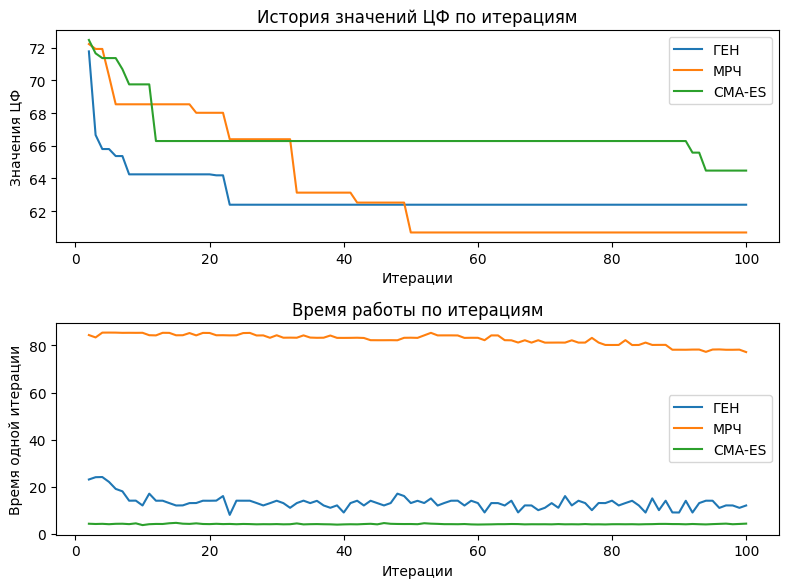
\includegraphics[height=0.38\textheight,valign=t]{my_folder/images//cost-history.png}
    
\captionsetup{justification=centering} %центрировать
\caption{График изменения значения ЦФ по итерациям}\label{fig:ch-wd}
\end{figure}

\begin{figure}[!htbp]
    \centering
    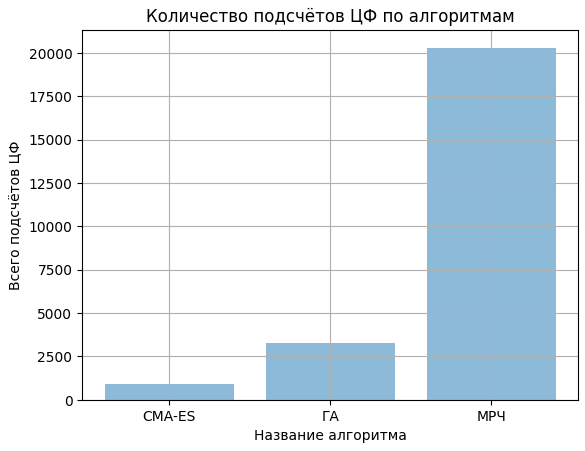
\includegraphics[height=0.38\textheight,valign=t]{my_folder/images//evalsall.png}
    
\captionsetup{justification=centering} %центрировать
\caption{Гистограмма, содержащая общее количество итераций $I$} \label{fig:hist-wd}
\end{figure}

\begin{figure}[!htbp]
    \centering
    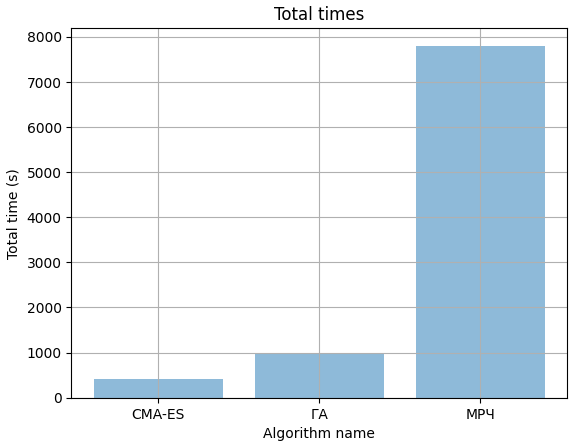
\includegraphics[height=0.38\textheight,valign=t]{my_folder/images//total-times.png}
    
\captionsetup{justification=centering} %центрировать
\caption{Гистограмма, содержащая общее время работы $T_{\text{общ}}$} \label{fig:hist-times-wd}
\end{figure}
\newpage
\section{Выводы} \label{ch4:conclusion}

По \taref{tab:opt-res} естественно заметить, что от эксперимента к эксперименту количество  хромосом, частиц, решений могло меняться для ГА, МРЧ, CMA-ES соответственно. Без потери смысловой нагрузки произведем сравнение подсчётов ЦФ в алгоритмах.\\
Поэтому разумно представить гиперпараметры, общие для всех вариантов запуска алгоритмов.\\
Гиперпараметры ГА при запуске:
\begin{itemize}
	\item Количество скрещивающихся родителей - половина от общего числа популяции.
	\item Мутация - случайная.
	\item Шанс мутации - $10\%$.
\end{itemize}
Гиперпараметры МРЧ при запуске:
\begin{itemize}
	\item $\omega = 0.5069$, $\varphi_p = 2.5524$, $\varphi_g = 1.0056$.
	\item $S = 203$.
\end{itemize}
Гиперпараметры CMA-ES при запуске:
\begin{itemize}
	\item $\sigma_0 = 5$.
	\item $X_0 = [65, 35, 20, 40, 22, 34]$. Здесь $X_0$ - начальное решение.
\end{itemize}
Из \taref{tab:opt-res} видно, что:
\begin{itemize}
	\item Лучшее решение было получено при помощи алгоритма МРЧ $f(X_{opt}) = 60.2$
	\item Лучшее решение МРЧ получено при установке гиперпараметров на основании \taref{tab:tab-pso-opt-params} с
	 $50\%$ увеличением количества подсчётов ЦФ.
	 \item Самое оптимальное решение, полученное при помощи МРЧ, требует в $\approx 13.5$ больше подсчётов ЦФ, чем самое оптимальное решение, полученное при помощи CMA-ES.
	 \item Самое оптимальное решение, полученное при помощи МРЧ, требует в $4.64$ раз больше подсчётов ЦФ, чем самое оптимальное решение, полученное при помощи ГЕН.
	 \item Самое оптимальное решение, полученное при помощи МРЧ, на $\approx 1.75\%$ лучше, чем самое оптимальное решение, полученное при помощи CMA-ES.
	 \item Самое оптимальное решение, полученное при помощи МРЧ, на $\approx 3.79\%$ лучше, чем самое оптимальное решение, полученное при помощи ГЕН.
	%\item МРЧ требует в $\approx 11.2$ раз больше подсчётов ЦФ по сравнению с CMA-ES, но выдаёт более %точное решение на $2,1\%$.
	\item В порядке использования вычислительно-временных ресурсов алгоритмы располагаются следующим образом :
	CMA-ES, ГА, МРЧ от лучшего к худшему.
	\item В порядке качества полученного решения алгоритмы располагаются 
	МРЧ, CMA-ES, ГА,  от лучшего к худшему.
\end{itemize}
Графики \firef{fig:ch-wd}, \firef{fig:hist-wd}, \firef{fig:hist-times-wd} построены на основании данных из \taref{tab:opt-res} при $I = 100$. График генетического алгоритма построен на данных, полученных при подсчёте ЦФ $f(X_{opt}) = 62.39$ из таблицы.\\
\firef{fig:ch-wd} является наглядным представлением требования МРЧ большого количества вычислительных ресурсов.
Результаты, полученные на выходе алгоритмов оптимизации в сравнении с \eqref{eq:src}, представляют возможность сделать следующие выводы:
\begin{itemize}
	\item Лучшее решение, полученное с помощью МРЧ, лучше исходного на $18 \%$.
	\item Лучшее решение, полученное с помощью CMA-ES, лучше исходного на $ 16.5\%$.
	\item Лучшее решение, полученное с помощью ГА, лучше исходного на $ 15\%$.
\end{itemize}
%% Вспомогательные команды - Additional commands
%
%\newpage % принудительное начало с новой страницы, использовать только в конце раздела
%\clearpage % осуществляется пакетом <<placeins>> в пределах секций
%\newpage\leavevmode\thispagestyle{empty}\newpage % 100 % начало новой страницы